\setcounter{chapter}{10}  % sets the current chapter to 10 so that the next one becomes 11

\chapter{Introduction to Hypothesis Testing}
\label{ch:intro-hypothesis}

\section{Test of Hypothesis for One Mean}

\begin{definition}[Hypothesis Tests]
An inferential procedure to determine whether there is sufficient evidence to suggest a condition for a population parameter using statistics from a sample.
\end{definition}


\textcolor{blue}{Attach a probability to the conclusion of a hypothesis test.}

\subsubsection*{Steps}
\begin{enumerate}
    \item Decide on a level of significance ($\alpha$)
    \item State the null hypothesis ($H_0$) and the alternative hypothesis ($H_a$) \textcolor{blue}{($H_1$)}
    \item Calculate the appropriate test statistic.
    \item Use the test statistic and a reference distribution to calculate a p-value. \\
    \textcolor{blue}{(Also refer back to $H_a$)}
    \item Compare p-value to $\alpha$ to make a conclusion.
\end{enumerate}

\textcolor{blue}{Note:} \\
\textcolor{blue}{The definition of a p-value can be confusing. We will define it later.}

\subsection*{Step 1: Decide on a Level of Significance ($\alpha$)}
-Threshold for decision making.

-Depends on tolerance for consequences of errors, sample size, nature of the study, and variability.

-Common values: $0.10$, $0.01$, $0.05$ \textcolor{blue}{(very common default)}

\subsection*{Step 2: State the Null Hypothesis ($H_0$) and the Alternative Hypothesis ($H_a$)}

\textbf{$\Theta$:} parameter of interest

\textbf{$\Theta_0$:} numerical value of the parameter of interest hypothesized under the null hypothesis.

\[
\begin{array}{lll}
H_0: \Theta = \Theta_0 & (\Theta \leq \Theta_0) & H_a: \Theta > \Theta_0 \quad \textcolor{blue}{\text{one-sided (one-tailed)}} \\
H_0: \Theta = \Theta_0 & (\Theta \geq \Theta_0) & H_a: \Theta < \Theta_0 \quad \textcolor{blue}{\text{one-sided (one-tailed)}} \\
H_0: \Theta = \Theta_0 &                         & H_a: \Theta \neq \Theta_0 \quad \textcolor{purple}{\text{two-sided (two-tailed)}}
\end{array}
\]


\textbf{Null ($H_0$):} Represents the current belief (\textcolor{blue}{status quo}) or the safe belief.

\textbf{Alternative ($H_a$):} Represents the research hypothesis (or what you are asked to test)
\subsection*{Step 3: Calculate an appropriate test statistic}

Depends on the hypothesis test conducted and the information available.


\begin{definition}[Test Statistic Skeleton]
\[
\text{test statistic} = \frac{\text{(a statistic)} - \text{(hypothesized value of parameters under } H_0 \text{)}}{\text{standard error of statistic}}
\]
\end{definition}

The test statistic follows a reference distribution ($Z$, $t$, $F$, $\chi^2$).
\subsection*{Step 4: Calculate the p-value}

\noindent
Use the test statistic, reference distribution, and refer back to $H_a$.

% --- BLUE: Right-tailed tests ---
\begin{figure}[H]
  \centering
  \begin{minipage}[t]{0.48\textwidth}
    \centering
    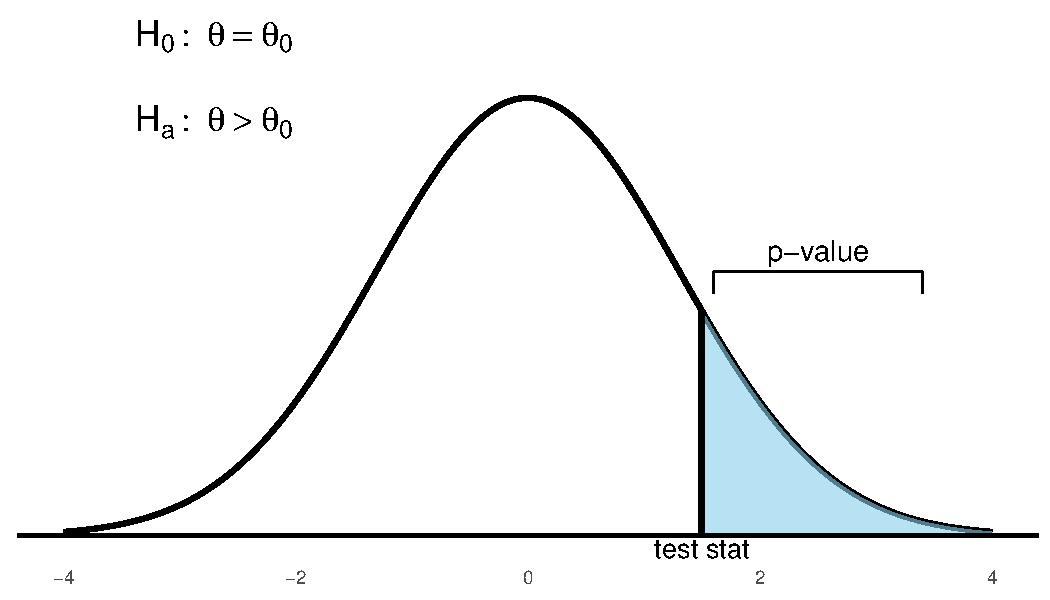
\includegraphics[width=\linewidth]{section11/images/hypothesis_right_tail.pdf}
  \end{minipage}
  \hfill
  \begin{minipage}[t]{0.48\textwidth}
    \centering
    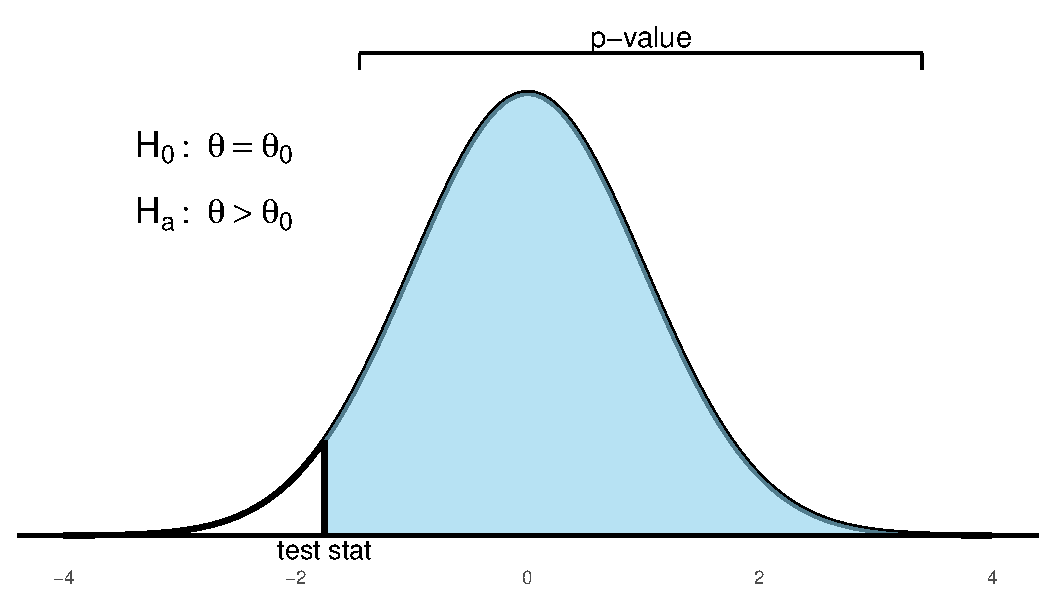
\includegraphics[width=\linewidth]{section11/images/hypothesis_right_tail_wide.pdf}
  \end{minipage}
  \caption*{Right-tailed test: \textit{p}-value is the area to the right of the test statistic.}
\end{figure}


% --- PINK: Left-tailed tests ---
\begin{figure}[H]
  \centering
  \begin{minipage}{0.48\textwidth}
    \centering
    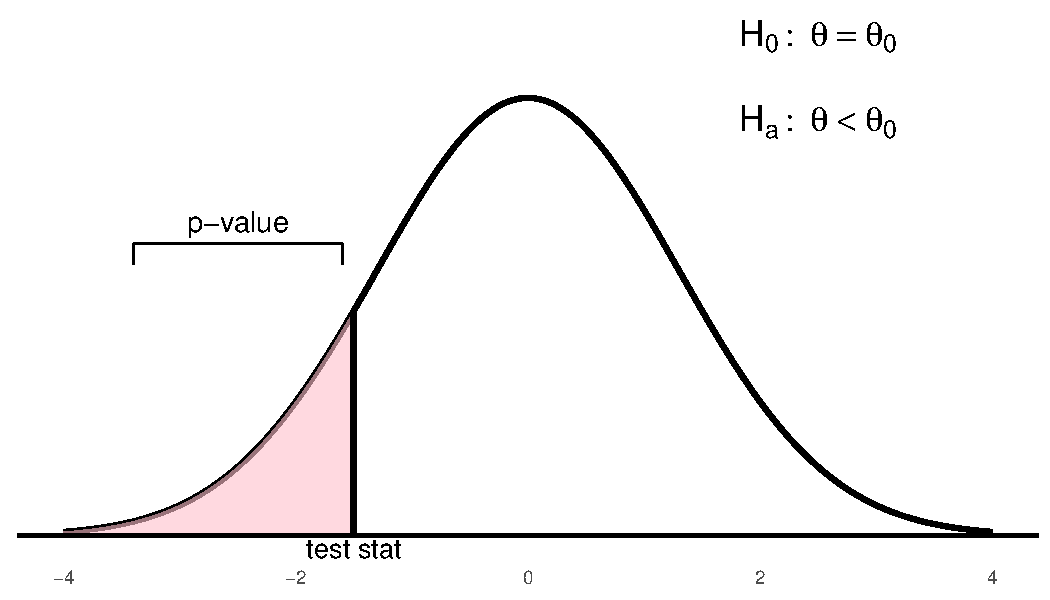
\includegraphics[width=\textwidth]{section11/images/hypothesis_left_tail.pdf}
  \end{minipage}
  \hfill
  \begin{minipage}{0.48\textwidth}
    \centering
    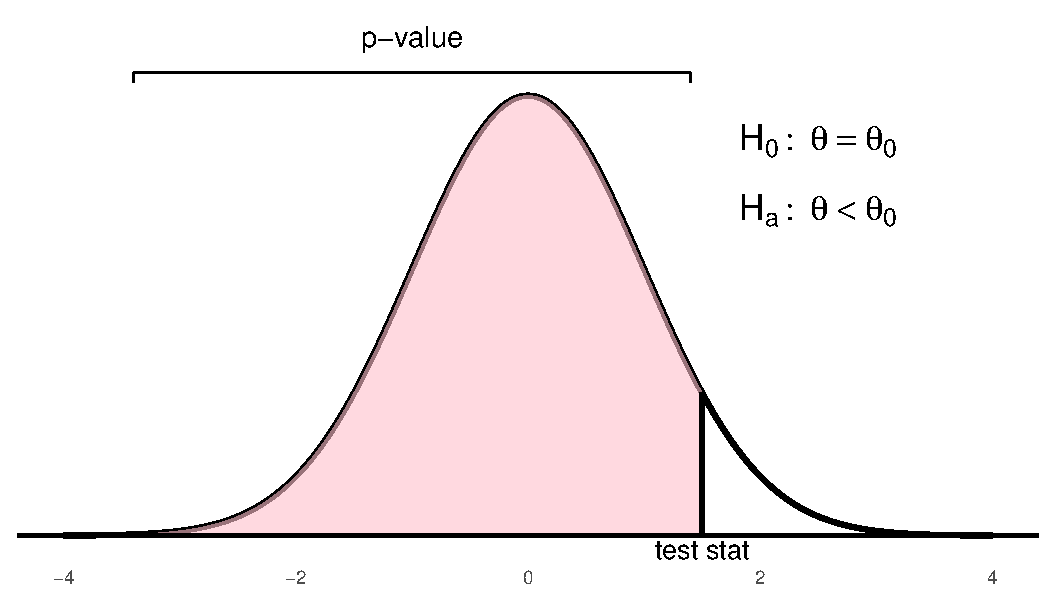
\includegraphics[width=\textwidth]{section11/images/hypothesis_left_tail_wide.pdf}
  \end{minipage}
\caption*{Left-tailed test: \textit{p}-value is the area to the left of the test statistic.}
\end{figure}

% --- GREEN: Two-tailed test ---
\begin{figure}[H]
  \centering
  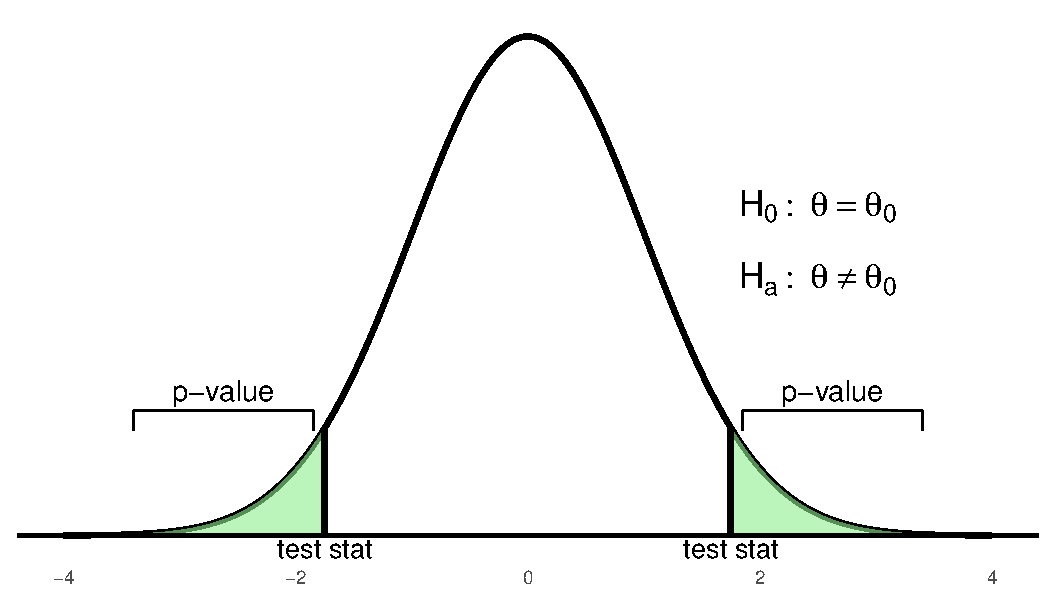
\includegraphics[width=0.52\textwidth]{section11/images/hypothesis_two_tail.pdf}
  \caption*{Two-tailed test: p-value is the total area in both tails beyond $\pm$ test statistic.}
\end{figure}



